

\tikzset{every picture/.style={line width=0.75pt}} %set default line width to 0.75pt        

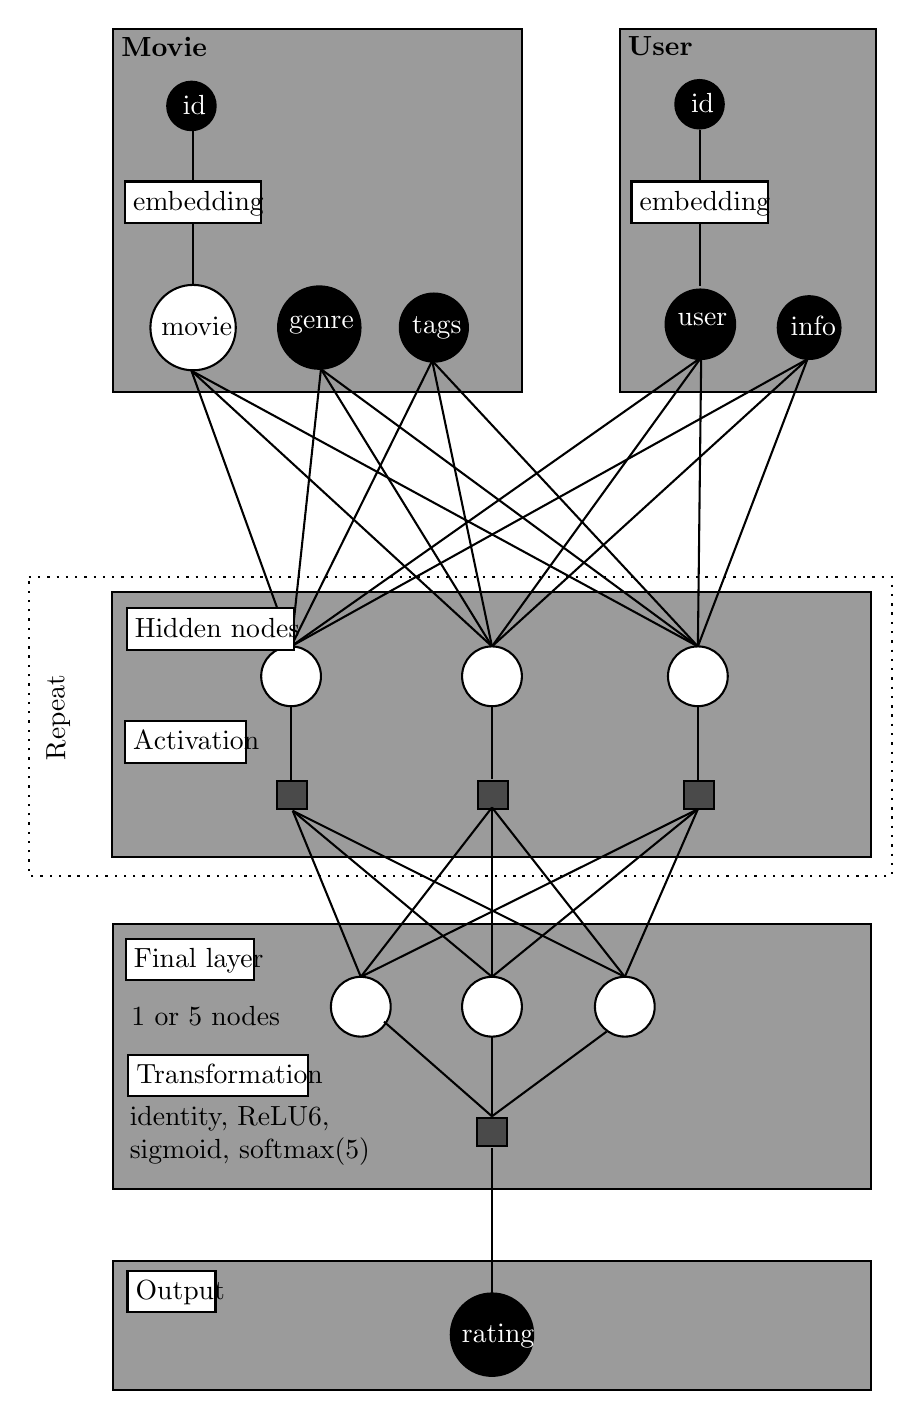
\begin{tikzpicture}[x=0.75pt,y=0.75pt,yscale=-1,xscale=1, scale=0.8]
%uncomment if require: \path (0,923); %set diagram left start at 0, and has height of 923


%Shape: Rectangle [id:dp2307314996446338] 
\draw  [fill={rgb, 255:red, 155; green, 155; blue, 155 }  ,fill opacity=1 ] (122,31) -- (368,31) -- (368,250) -- (122,250) -- cycle ;
%Straight Lines [id:da16141207798725943] 
\draw    (170,92) -- (170,123) ;
%Straight Lines [id:da256251158457261] 
\draw    (170,148) -- (170,186) ;
%Shape: Rectangle [id:dp4062601423389237] 
\draw  [fill={rgb, 255:red, 155; green, 155; blue, 155 }  ,fill opacity=1 ] (427,31) -- (581,31) -- (581,250) -- (427,250) -- cycle ;
%Straight Lines [id:da5944797488705584] 
\draw    (475,92) -- (475,123) ;
%Straight Lines [id:da3036173249772247] 
\draw    (475,148) -- (475,186) ;
%Shape: Rectangle [id:dp9997854452663028] 
\draw  [fill={rgb, 255:red, 155; green, 155; blue, 155 }  ,fill opacity=1 ] (121,370) -- (578,370) -- (578,530) -- (121,530) -- cycle ;
%Straight Lines [id:da5917985818254904] 
\draw    (169,237) -- (229,403) ;
%Shape: Circle [id:dp6114587760100195] 
\draw  [fill={rgb, 255:red, 255; green, 255; blue, 255 }  ,fill opacity=1 ] (332,421) .. controls (332,411.06) and (340.06,403) .. (350,403) .. controls (359.94,403) and (368,411.06) .. (368,421) .. controls (368,430.94) and (359.94,439) .. (350,439) .. controls (340.06,439) and (332,430.94) .. (332,421) -- cycle ;
%Shape: Circle [id:dp553345531736126] 
\draw  [fill={rgb, 255:red, 255; green, 255; blue, 255 }  ,fill opacity=1 ] (456,421) .. controls (456,411.06) and (464.06,403) .. (474,403) .. controls (483.94,403) and (492,411.06) .. (492,421) .. controls (492,430.94) and (483.94,439) .. (474,439) .. controls (464.06,439) and (456,430.94) .. (456,421) -- cycle ;
%Shape: Circle [id:dp16008652747984975] 
\draw  [fill={rgb, 255:red, 255; green, 255; blue, 255 }  ,fill opacity=1 ] (211,421) .. controls (211,411.06) and (219.06,403) .. (229,403) .. controls (238.94,403) and (247,411.06) .. (247,421) .. controls (247,430.94) and (238.94,439) .. (229,439) .. controls (219.06,439) and (211,430.94) .. (211,421) -- cycle ;
%Straight Lines [id:da07936131606411578] 
\draw    (169,237) -- (474,403) ;
%Straight Lines [id:da03140198678455175] 
\draw    (169,237) -- (350,403) ;
%Straight Lines [id:da8972801381289985] 
\draw    (247,236) -- (229,403) ;
%Straight Lines [id:da5048950093422406] 
\draw    (247,236) -- (474,403) ;
%Straight Lines [id:da2676023756738023] 
\draw    (247,236) -- (350,403) ;
%Straight Lines [id:da4547393022990093] 
\draw    (314,231) -- (229,403) ;
%Straight Lines [id:da6479494477610002] 
\draw    (314,231) -- (474,403) ;
%Straight Lines [id:da443095768705153] 
\draw    (314,231) -- (350,403) ;
%Straight Lines [id:da35507587145535247] 
\draw    (476,229) -- (424.1,265.56) -- (229,403) ;
%Straight Lines [id:da9486617458047818] 
\draw    (476,229) -- (474,403) ;
%Straight Lines [id:da8058732839276246] 
\draw    (476,229) -- (350,403) ;
%Straight Lines [id:da8260388432043336] 
\draw    (540,230) -- (229,403) ;
%Straight Lines [id:da9400545257458622] 
\draw    (540,230) -- (474,403) ;
%Straight Lines [id:da05542791968584537] 
\draw    (540,230) -- (350,403) ;
%Shape: Rectangle [id:dp27962627521584915] 
\draw  [dash pattern={on 0.84pt off 2.51pt}] (71,361) -- (591,361) -- (591,541) -- (71,541) -- cycle ;
%Shape: Rectangle [id:dp7643196245006507] 
\draw  [fill={rgb, 255:red, 155; green, 155; blue, 155 }  ,fill opacity=1 ] (121.5,570) -- (578.5,570) -- (578.5,730) -- (121.5,730) -- cycle ;
%Shape: Circle [id:dp2621970126778864] 
\draw  [fill={rgb, 255:red, 255; green, 255; blue, 255 }  ,fill opacity=1 ] (332,620) .. controls (332,610.06) and (340.06,602) .. (350,602) .. controls (359.94,602) and (368,610.06) .. (368,620) .. controls (368,629.94) and (359.94,638) .. (350,638) .. controls (340.06,638) and (332,629.94) .. (332,620) -- cycle ;
%Shape: Rectangle [id:dp18515621761343992] 
\draw  [fill={rgb, 255:red, 155; green, 155; blue, 155 }  ,fill opacity=1 ] (121.5,773) -- (578.5,773) -- (578.5,851) -- (121.5,851) -- cycle ;
%Straight Lines [id:da013824347109618329] 
\draw    (229,484) -- (229,439) ;
%Straight Lines [id:da10108684835813209] 
\draw    (474,484) -- (474,439) ;
%Straight Lines [id:da4795087140136396] 
\draw    (350,483) -- (350,439) ;
%Shape: Rectangle [id:dp9994780808740696] 
\draw  [fill={rgb, 255:red, 74; green, 74; blue, 74 }  ,fill opacity=1 ] (220.5,484) -- (238.5,484) -- (238.5,501) -- (220.5,501) -- cycle ;
%Shape: Rectangle [id:dp4560542280088048] 
\draw  [fill={rgb, 255:red, 74; green, 74; blue, 74 }  ,fill opacity=1 ] (341.5,484) -- (359.5,484) -- (359.5,501) -- (341.5,501) -- cycle ;
%Shape: Rectangle [id:dp1716916612978231] 
\draw  [fill={rgb, 255:red, 74; green, 74; blue, 74 }  ,fill opacity=1 ] (465.5,484) -- (483.5,484) -- (483.5,501) -- (465.5,501) -- cycle ;
%Shape: Circle [id:dp45715525538322044] 
\draw  [fill={rgb, 255:red, 255; green, 255; blue, 255 }  ,fill opacity=1 ] (412,620) .. controls (412,610.06) and (420.06,602) .. (430,602) .. controls (439.94,602) and (448,610.06) .. (448,620) .. controls (448,629.94) and (439.94,638) .. (430,638) .. controls (420.06,638) and (412,629.94) .. (412,620) -- cycle ;
%Shape: Circle [id:dp6321049451181513] 
\draw  [fill={rgb, 255:red, 255; green, 255; blue, 255 }  ,fill opacity=1 ] (253,620) .. controls (253,610.06) and (261.06,602) .. (271,602) .. controls (280.94,602) and (289,610.06) .. (289,620) .. controls (289,629.94) and (280.94,638) .. (271,638) .. controls (261.06,638) and (253,629.94) .. (253,620) -- cycle ;
%Straight Lines [id:da32751333097955326] 
\draw    (271,602) -- (230,502) ;
%Straight Lines [id:da8245521872295072] 
\draw    (350,602) -- (350,500) ;
%Straight Lines [id:da56525565956782] 
\draw    (430,602) -- (474,501) ;
%Shape: Rectangle [id:dp24794467141710175] 
\draw  [fill={rgb, 255:red, 74; green, 74; blue, 74 }  ,fill opacity=1 ] (341,687) -- (359,687) -- (359,704) -- (341,704) -- cycle ;
%Straight Lines [id:da5299916115667694] 
\draw    (285,629) -- (350,686) ;
%Straight Lines [id:da556666846670562] 
\draw    (350,638) -- (350,686) ;
%Straight Lines [id:da19442212012957627] 
\draw    (419,635) -- (350,686) ;
%Straight Lines [id:da9110766057280562] 
\draw    (350,793) -- (350,705) ;
%Straight Lines [id:da4082820567804806] 
\draw    (350,602) -- (230,502) ;
%Straight Lines [id:da6303177546387124] 
\draw    (430,602) -- (230,502) ;
%Straight Lines [id:da11911691336503638] 
\draw    (430,602) -- (350,500) ;
%Straight Lines [id:da3514741732937119] 
\draw    (271,602) -- (350,500) ;
%Straight Lines [id:da8869392440246155] 
\draw    (350,602) -- (474,501) ;
%Straight Lines [id:da22608196348921028] 
\draw    (271,602) -- (474,501) ;

% Text Node
\draw (125,34) node [anchor=north west][inner sep=0.75pt]   [align=left] {\textbf{Movie}};
% Text Node
\draw  [fill={rgb, 255:red, 0; green, 0; blue, 0 }  ,fill opacity=1 ]  (169, 77.5) circle [x radius= 14.6, y radius= 14.6]   ;
\draw (162,69) node [anchor=north west][inner sep=0.75pt]  [color={rgb, 255:red, 255; green, 255; blue, 255 }  ,opacity=1 ] [align=left] {id};
% Text Node
\draw  [fill={rgb, 255:red, 0; green, 0; blue, 0 }  ,fill opacity=1 ]  (246, 211) circle [x radius= 24.82, y radius= 24.82]   ;
\draw (226,202.5) node [anchor=north west][inner sep=0.75pt]  [color={rgb, 255:red, 255; green, 255; blue, 255 }  ,opacity=1 ] [align=left] {genre};
% Text Node
\draw  [fill={rgb, 255:red, 0; green, 0; blue, 0 }  ,fill opacity=1 ]  (315, 211) circle [x radius= 20.52, y radius= 20.52]   ;
\draw (300,202.5) node [anchor=north west][inner sep=0.75pt]  [color={rgb, 255:red, 255; green, 255; blue, 255 }  ,opacity=1 ] [align=left] {tags};
% Text Node
\draw  [fill={rgb, 255:red, 255; green, 255; blue, 255 }  ,fill opacity=1 ]  (129,123) -- (211,123) -- (211,148) -- (129,148) -- cycle  ;
\draw (132,127) node [anchor=north west][inner sep=0.75pt]   [align=left] {embedding};
% Text Node
\draw  [fill={rgb, 255:red, 255; green, 255; blue, 255 }  ,fill opacity=1 ]  (170, 211) circle [x radius= 25.71, y radius= 25.71]   ;
\draw (149,202.5) node [anchor=north west][inner sep=0.75pt]   [align=left] {movie};
% Text Node
\draw (430,34) node [anchor=north west][inner sep=0.75pt]   [align=left] {\textbf{User}};
% Text Node
\draw  [fill={rgb, 255:red, 0; green, 0; blue, 0 }  ,fill opacity=1 ]  (475, 76.5) circle [x radius= 14.6, y radius= 14.6]   ;
\draw (468,68) node [anchor=north west][inner sep=0.75pt]  [color={rgb, 255:red, 255; green, 255; blue, 255 }  ,opacity=1 ] [align=left] {id};
% Text Node
\draw  [fill={rgb, 255:red, 0; green, 0; blue, 0 }  ,fill opacity=1 ]  (541, 211) circle [x radius= 18.9, y radius= 18.9]   ;
\draw (528,202.5) node [anchor=north west][inner sep=0.75pt]  [color={rgb, 255:red, 255; green, 255; blue, 255 }  ,opacity=1 ] [align=left] {info};
% Text Node
\draw  [fill={rgb, 255:red, 255; green, 255; blue, 255 }  ,fill opacity=1 ]  (434,123) -- (516,123) -- (516,148) -- (434,148) -- cycle  ;
\draw (437,127) node [anchor=north west][inner sep=0.75pt]   [align=left] {embedding};
% Text Node
\draw  [fill={rgb, 255:red, 0; green, 0; blue, 0 }  ,fill opacity=1 ]  (475.5, 209) circle [x radius= 20.94, y radius= 20.94]   ;
\draw (460,200.5) node [anchor=north west][inner sep=0.75pt]  [color={rgb, 255:red, 255; green, 255; blue, 255 }  ,opacity=1 ] [align=left] {user};
% Text Node
\draw  [fill={rgb, 255:red, 255; green, 255; blue, 255 }  ,fill opacity=1 ]  (130,380) -- (231,380) -- (231,405) -- (130,405) -- cycle  ;
\draw (133,384) node [anchor=north west][inner sep=0.75pt]   [align=left] {Hidden nodes};
% Text Node
\draw (79.86,473.62) node [anchor=north west][inner sep=0.75pt]  [rotate=-269.18] [align=left] {Repeat};
% Text Node
\draw  [fill={rgb, 255:red, 255; green, 255; blue, 255 }  ,fill opacity=1 ]  (129.5,579) -- (206.5,579) -- (206.5,604) -- (129.5,604) -- cycle  ;
\draw (132.5,583) node [anchor=north west][inner sep=0.75pt]   [align=left] {Final layer};
% Text Node
\draw  [fill={rgb, 255:red, 255; green, 255; blue, 255 }  ,fill opacity=1 ]  (131,649) -- (239,649) -- (239,674) -- (131,674) -- cycle  ;
\draw (134,653) node [anchor=north west][inner sep=0.75pt]   [align=left] {Transformation};
% Text Node
\draw  [fill={rgb, 255:red, 255; green, 255; blue, 255 }  ,fill opacity=1 ]  (130.5,779) -- (183.5,779) -- (183.5,804) -- (130.5,804) -- cycle  ;
\draw (133.5,783) node [anchor=north west][inner sep=0.75pt]   [align=left] {Output};
% Text Node
\draw  [fill={rgb, 255:red, 0; green, 0; blue, 0 }  ,fill opacity=1 ]  (350, 817.5) circle [x radius= 24.82, y radius= 24.82]   ;
\draw (330,809) node [anchor=north west][inner sep=0.75pt]  [color={rgb, 255:red, 255; green, 255; blue, 255 }  ,opacity=1 ] [align=left] {rating};
% Text Node
\draw (130,678) node [anchor=north west][inner sep=0.75pt]   [align=left] {identity, ReLU6, \\sigmoid, softmax(5)};
% Text Node
\draw (131,618) node [anchor=north west][inner sep=0.75pt]   [align=left] {1 or 5 nodes};
% Text Node
\draw  [fill={rgb, 255:red, 255; green, 255; blue, 255 }  ,fill opacity=1 ]  (129,448) -- (202,448) -- (202,473) -- (129,473) -- cycle  ;
\draw (132,452) node [anchor=north west][inner sep=0.75pt]   [align=left] {Activation};


\end{tikzpicture}

